\documentclass[11pt]{article}
\usepackage[margin=1in]{geometry}
\usepackage{amsmath,amssymb,booktabs,longtable,graphicx,hyperref}
\usepackage{array}
\hypersetup{colorlinks=true,linkcolor=blue,urlcolor=blue}
\emergencystretch=2em

\newcommand{\code}[1]{\texttt{\detokenize{#1}}}
\newcommand{\E}{\mathrm{E}}
\renewcommand{\thesection}{S\arabic{section}}
\renewcommand{\thetable}{S\arabic{table}}
\renewcommand{\thefigure}{S\arabic{figure}}

\title{Supplementary Material for\\
Learning Time Transformations for Stiff Hamiltonian Systems:\\
Deployment Reliability and Applicability Boundaries}
\author{\begin{tabular}{c}
Jiangshan Wang\textsuperscript{a}, Shuxiang Xu\textsuperscript{b},
Shuai Zhu\textsuperscript{c,*}\\[0.5em]
\small\textsuperscript{a}Department of Emergency and Trauma, The First Affiliated Hospital\\
\small of Naval Medical University, Shanghai, China\\
\small\textsuperscript{b}College of Mechanical Engineering, Guizhou University, Guiyang, China\\
\small\textsuperscript{c}Shanghai Iluvatar CoreX Semiconductor Co., Ltd., Shanghai, China\\[0.5em]
\small\textsuperscript{*}Corresponding author: Shuai Zhu;
\href{mailto:zhushuaisjtu@gmail.com}{\small zhushuaisjtu@gmail.com}
\end{tabular}}
\date{}

\begin{document}
\maketitle
\tableofcontents

\section{Purpose and artifact authority}

This supplement records implementation and protocol details for the
accompanying manuscript, including the definitions needed to reproduce
its denominators and comparisons. The main text gives the scientific
interpretation.

The study contains two distinct evidence channels. The primary channel uses
the exact Kepler Hamiltonian and evaluates learned monitors as deployed by a
finite implicit solver. A separate learned-Hamiltonian gate tests whether a
candidate Hamiltonian is sufficiently faithful for deployment; because no
candidate passes that gate, it supplies no learned-H downstream rollout
results. The modal and Duffing calculations are finite scope checks.

All numerical records retain failed evaluations in their denominators.
Checkpoint, orbit and scenario identifiers are shared within a training
recipe where stated; they are not independent draws from a deployment
population. Internal source files, hashes and local evidence maps are listed
in the release manifest accompanying this supplement.

\begin{table}[ht]
\centering\small
\caption{Notation for the Hamiltonian time transformation and its numerical
realisation. All gradients in $z$ use the canonical ordering $(q,p)$.}
\label{tab:notation}
\begin{tabular}{@{}ll@{}}
\toprule
Symbol & Meaning \\
\midrule
$z=(q,p)$; $d$ & Physical phase point; configuration dimension \\
$H$; $\widehat H$ & True Hamiltonian; Hamiltonian supplied to the integrator \\
$\psi$; $\theta$ & Hamiltonian parameters; monitor parameters \\
$t$; $\tau$ & Physical time; transformed time \\
$p_0$ & Momentum conjugate to $t$, fixed at $-\widehat H(z_0)$ \\
$g_\theta$; $c_\theta$ & Positive monitor; bounded multiplicative correction \\
$K_\theta$; $F_\theta$ & Extended Hamiltonian; state vector field in $\tau$ \\
$h_n$; $\bar z_n$ & Transformed-time step; endpoint midpoint \\
$R_n$; $u_k$; $r_k$ & Endpoint residual; update norm; returned residual norm \\
$r$; $L$; $\phi$ & Kepler radius; angular momentum; invariant features \\
$s_j$; $T$ & Training checkpoint time; deployment physical horizon \\
\bottomrule
\end{tabular}
\end{table}

\section{Numerical construction}

\subsection{Extended Hamiltonian and endpoint solve}

For canonical state $z=(q,p)$, the deployed construction is
\[
 K(z,p_0)=g_\theta(z)\,[\widehat H(z)+p_0],
 \qquad p_0=-\widehat H(z_0).
\]
The transformed dynamics are advanced with implicit midpoint. Each endpoint
starts from the explicit predictor and is updated by the recorded fixed-point
iteration. Completion is determined by the implementation's update-based
stopping rule and iteration budget. The historical returned-residual replay
covers 1748 baseline/control/refinement evaluations. A separate current
review covers all 252 step interventions and 1080 new training-arm
evaluations, first under the original stopping rule and then with verified
returned-residual acceptance. The latter requires an update below
$10^{-12}$ to trigger verification and a returned residual below
$10^{-12}$ to accept, within the original 100 iterations. Reported
intervention completion uses this successor.

The terminal physical-time search uses a finite bisection procedure. The
reported clock is set to the target horizon after the final candidate is
selected. Therefore a recorded zero terminal-time error is not an
independent measurement of the selected candidate's clock error. Exact
symplecticity of a prescribed, state-independent implicit midpoint map is
also not assigned to finite solver iterations or to this state-dependent
terminal procedure.

\subsection{Monitor families}

The baseline monitors use either raw state inputs or invariant features. The
positive output is produced by a bounded sigmoid parameterisation. The
factorised monitor used in the structural intervention is
\[
 g_\theta(q,p)=r(q)\,2\sigma\!\left(N_\theta(\phi(q,p))\right),
 \qquad r(q)=\lVert q\rVert,
\]
so its value lies between zero and $2r$ for finite network output. This
output bound does not bound all monitor derivatives and does not by itself
imply endpoint convergence. The factorised and unfactorised arms also differ
in output bias, state generation, validation aggregation and non-finite
handling; they are complete recipe comparisons rather than a single-factor
ablation.

Training uses finite unrolled endpoint updates and detached clock
interpolation weights. The resulting objective is not identical to a fully
converged implicit deployment calculation. Validation loss is therefore
reported as a training diagnostic, not as a solver-reliability certificate.

\subsection{Kepler training and validation}

The scalar network has two hidden layers of width 64 with hyperbolic
tangent activations. Raw inputs are $(q,p)$; invariant inputs are
$(r,r^{-1},\lVert p\rVert^2,(q\cdot p)^2,L^2)$, with
$L=q_1p_2-q_2p_1$. The output is $2\sigma(f_\theta)$ for unfactored
monitors and $2r\sigma(f_\theta)$ for factored monitors. Final-layer
weights have a normal distribution of standard deviation 0.1; final-layer
biases are $-2.2$ and 0, respectively. Thus a zero factored bias does not
give an initially constant correction.

Each rollout uses $N=100$ transformed steps at $h=0.08$, with an explicit
predictor followed by four fixed-point updates per endpoint. The objective
in the main text uses weights $(w_E,w_z,\lambda_g)=(0.1,5,0.02)$.
Physical-time checkpoints are $s_j=0.3j$ relative to the sampled start.
Only times strictly below the attained clock are included, and the
checkpoint term is zero if none are attained. Linear interpolation uses
brackets and weights computed from detached clocks. Gradients pass through
endpoint states, but not through interpolation weights or checkpoint
selection.

Adam starts at learning rate $2\times10^{-4}$, with cosine decay over
600 epochs and gradient-norm clipping at 1. Each epoch samples one start
from 4096 equally spaced mean anomalies, with probabilities proportional
to $(r^{3/2}+0.05)^{-1}$. Validation uses eight fixed initial anomalies
every 50 epochs; checkpoint selection minimises validation state MSE.
The training orbit has $a=1$ and $e=0.9$ for the baseline, and $e=0.99$
for the expanded-domain arm.

Baseline validation pools errors across checkpoint times and initial
states. New-arm validation first averages within each initial-state
rollout, then across the eight starts. New arms also use safeguarded
Kepler-equation state generation and skip and count non-finite loss or
gradient-norm epochs. Four epochs are skipped in one factored $e=0.99$
run and none in the other new arms. These differences accompany
factorisation and remain part of the recipe comparison. Both training
orbits leave the smallest deployment periapsis, 0.0075, uncovered.

The architecture--solver control instead distils five students per input
architecture from one frozen teacher. It fits monitor outputs by MSE on
4096 states of the $a=1$, $e=0.9$ orbit, reserving every fourth state for
validation. Its shared teacher is distinct from the independently
rollout-trained checkpoints.

\section{Systems and evaluation grids}

\subsection{Kepler deployment}

Five independently trained checkpoints per baseline family are evaluated
on the Cartesian grid
\[
\begin{aligned}
a&\in\{0.75,1,1.25\}, & e&\in\{0.7,0.9,0.99\},\\
M_0&\in\{\pi,\pi/2\}, & \alpha&\in\{0,\pi/2\}, &
\eta&\in\{+1,-1\}.
\end{aligned}
\]
Here $M_0$ is mean anomaly, $\alpha$ the common position--momentum
rotation, and $\eta$ the momentum direction. Each checkpoint has
72 scenarios, giving 720 baseline learned evaluations and 72 manual
$g=r$ controls. The horizon is $T=2\pi a^{3/2}$, transformed step
$h=0.04$, update-based tolerance $10^{-12}$, maximum 100 fixed-point
updates per endpoint and accepted-step cap $10^5$.
The three new arms each have five matched seed identities and the same
grid, giving 1080 additional evaluations.

The highest-eccentricity cases have a smaller periapsis than the training
orbit. This is a finite-radius deployment test, not a limit as $r\to0$ and
not a collision-regularisation experiment.

\subsection{Reference diagnostic and intervention}

The reference diagnostic samples analytic Kepler ellipses at 720 states per
orbit and evaluates the endpoint Jacobian of the extended Hamiltonian with
automatic differentiation. Its maximum spectral-radius statistic is paired
with known completion labels in the retrospective comparison. Failure
locations are obtained by projecting recorded failure times onto the
analytic reference orbit; they are not direct observations of failed
iterates.

The step intervention selects all 252 failed baseline learned rollouts
and retains their checkpoints and scenarios. It uses
\[
h_{\rm test}=h\min\!\left(1,\frac{0.5}{\rho_{\max}^{\rm ref}}\right),
\]
with no change for a zero statistic, and increases the accepted-step cap
to $2\times10^6$. The per-endpoint fixed-point rule remains unchanged.
The initial diagnostic comparison uses already known completion labels;
development pilots and a resealed execution after a filesystem failure
belong to its protocol history. In the new-arm study, each full diagnostic
finishes before that checkpoint's deployment evaluations. This is
prospective use on new checkpoints on an informed, fixed grid. Short
training and pipeline pilots are excluded from outcomes.

The distilled solver control uses apoapsis starts, $a=1$, the same three
eccentricities, two orientations and two momentum directions, with
$T=3P(1)$ and $h=0.04$. These counts are kept separate from the principal
one-period, rollout-trained study.

\subsection{Non-Kepler scope checks}

The modal system has 16 modes and 32 canonical state variables, with tested
frequency ratios 10 and 20. Its implemented modal dynamics remain separable
in modal coordinates. The Duffing check has two state variables. These
systems test finite execution, accuracy and work bookkeeping; they do not
constitute evidence for large coupled stiff Hamiltonians.

\subsection{Classical controls and solver settings}

The Kepler accuracy--cost sweep retains only $\alpha=0$ and $\eta=+1$
from the main grid, giving 18 scenarios per configuration. Direct
physical-time midpoint uses steps 0.02, 0.01 and 0.005. Step-doubling
adaptive midpoint uses relative tolerances $10^{-5}$ and $10^{-7}$,
with absolute tolerance $10^{-12}$. Manual and ten baseline learned
monitors use transformed steps 0.08, 0.04 and 0.02, giving 38 configurations
and 684 evaluations. Newly factored arms are outside this sweep.

The adaptive controller compares one full midpoint step with two half
steps, divides their state difference by 3 and uses a root-mean-square
component error scaled by absolute and relative tolerances. It returns
the two-half-step state on acceptance and retains rejected-trial work.
Physical-time endpoint solves use tolerance $10^{-13}$; transformed
fixed-point solves use $10^{-12}$, with at most 100 updates.
The distilled Newton control permits 12 iterations, eight backtracks and
minimum damping $2^{-8}$, checking the defining residual at the returned
trial endpoint.

Non-Kepler controls use velocity Verlet at physical step 0.001 and
midpoint with prescribed monitor $0.75+0.25/(1+\lVert u\rVert^2/16)$
for the modal system and $0.75+0.25/(1+x^2)$ for Duffing.
Full-horizon reference refinement compares steps 0.002, 0.001 and 0.0005
on all 36 scenarios. The finest reference retains positive estimated
uncertainty; Richardson estimates are not rigorous bounds.

\subsection{Learned-Hamiltonian fidelity gate}

Five independently initialised candidates are fitted to Hamiltonian
gradients. Held-out eccentricities are $\{0.7,0.75,0.85,0.95,0.99\}$,
each with 257 phase-shifted states. Acceptance requires finite predictions
and the thresholds below for gradients and canonical vector fields.
\begin{center}
\begin{tabular}{lr}
\toprule
Metric & Maximum permitted value\\
\midrule
Overall normalised RMSE & 0.01\\
Normalised RMSE within each eccentricity stratum & 0.02\\
Pointwise relative-error 95th percentile & 0.03\\
Pointwise relative-error maximum & 0.15\\
\bottomrule
\end{tabular}
\end{center}
Normalised RMSE divides RMS prediction error by RMS target. Pointwise
relative error divides the error norm by the target norm, with a
$10^{-15}$ denominator floor. Multiplication by canonical $J$ preserves
Euclidean norms, so gradient and vector-field metrics are equivalent
here. At least three accepted candidates are required before downstream
monitor training and the planned solver comparison.

\section{Complete counts and primary outcomes}

\subsection{Early accepted-iterate conditioning: a negative result}
\label{sec:early-conditioning}

The corrected audit contains 1056 recorded rollouts: 264 from the
single-teacher architecture--solver study and 792 from independently
rollout-trained baselines and manual controls. There are 716 eventual
completions and 340 solver failures. At each accepted step index 10, 50
and 100, exactly one stored midpoint observation is selected per rollout.
Repeated within-rollout samples are not counted as independent
observations. Shared checkpoints and scenarios still induce dependence;
these pooled distributions are descriptive, not population inference.

In canonical planar ordering, let
$S=\operatorname{diag}(a,a,a^{-1/2},a^{-1/2})$ and
$B=S^{-1}JD^2_{zz}KS$. For each saved midpoint and its actual transformed
step $h$, the corrected operators are
\[
 D\widetilde R=I-\frac h2 B,\qquad
 q_{\mathrm{fp}}=\frac h2\|B\|_2.
\]
The singular values and Euclidean condition number refer to
$D\widetilde R$. The coefficient is $h$, without an additional
$a^{-3/2}$ factor: changing state coordinates by similarity does not
change the time variable. This audit supersedes the earlier incorrectly
scaled, repeated-observation diagnostic; its original artifacts are
retained solely as correction history.

At all three indices, failures have smaller median $q_{\mathrm{fp}}$
and condition number and larger median minimum singular value. At
step 100 the respective completed/failed medians are
0.00729855/0.00633913, 1.00957/1.00782 and 0.995238/0.996107.
Figure~\ref{fig:early-conditioning} retains the original corrected plot.
The contrasts do not support the hypothesised early association on this
grid. They neither rule out late endpoint difficulty nor show that no
other online diagnostic can work. A matched accepted-step index is not
a matched physical time or orbital phase; fixed-point and Newton
protocols are pooled here only for the recorded descriptive comparison.

\begin{figure}[ht]
\centering
\includegraphics[width=\textwidth]{../results/expAC14/conditioning_association.pdf}
\caption{Corrected conditioning at accepted step 100, reusing the original
audit figure. Each metric has 716 observations from eventual completions
and 340 from failures, one per recorded rollout. Outliers are suppressed
by the original boxplot display, not removed from the numerical summaries.
Checkpoint and scenario dependence remains. The observed directions do
not support early failure discrimination by these pooled local metrics.}
\label{fig:early-conditioning}
\end{figure}

\subsection{Architecture--solver comparison}
\label{sec:solver-comparison}

Five distilled students per architecture share one frozen teacher.
Each solver is evaluated on 60 scenarios per learned architecture and
12 manual controls, giving 264 runs across both solvers. Raw completion
changes from 30/60 to 34/60; invariant completion is 44/60 under each
solver. For invariant students, 40 scenarios complete under both, four
only under each solver and twelve under neither. These are three-period
evaluations, distinct from the one-period rollout-trained grid.
Figure~\ref{fig:solver-comparison} preserves the original comparison;
its rollout-level Wilson intervals do not estimate uncertainty across
an independently sampled checkpoint population. The associated
symmetry-error summaries are conditioned on all four transforms completing
and therefore do not measure unconditional deployment accuracy.
For the invariant students, energy and closure max/min ratios across
completed four-transform groups differ from one by at most
$4\times10^{-11}$. The raw-student maxima reach 637 and 695,
respectively. These ratios measure consistency on completed groups,
not an accuracy advantage on the full grid.

\begin{figure}[ht]
\centering
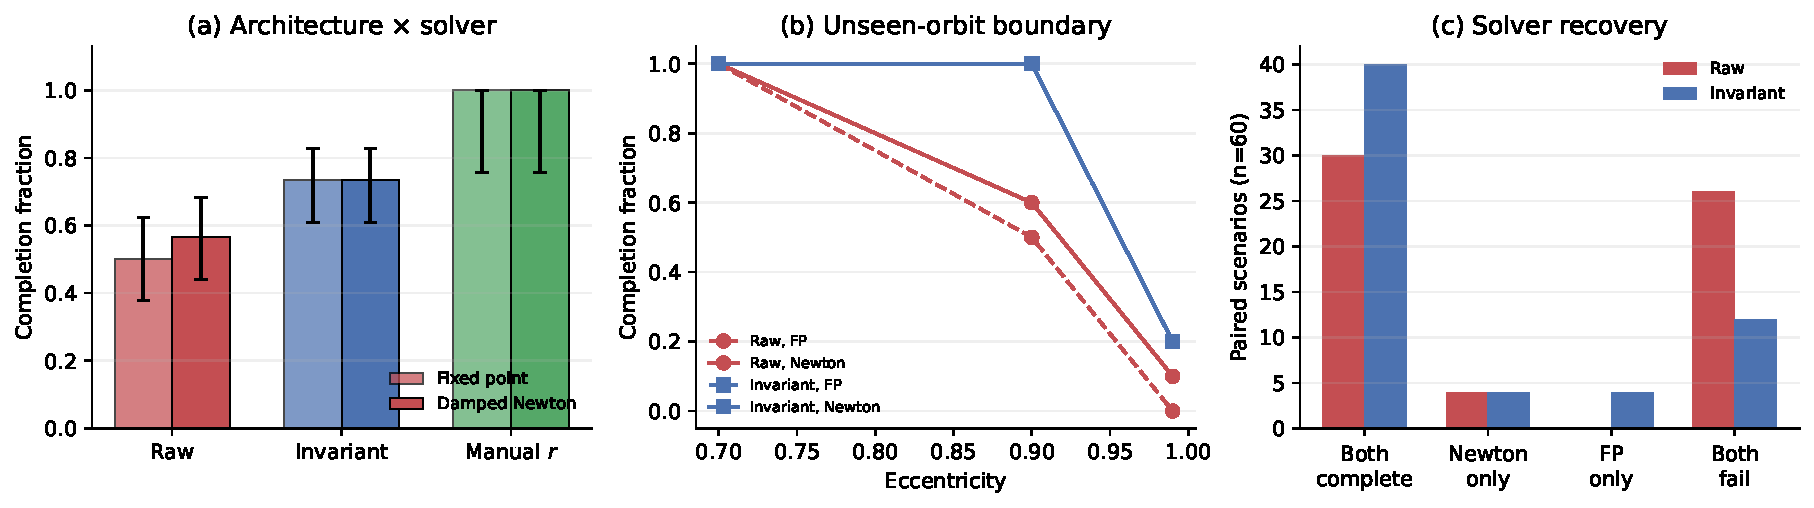
\includegraphics[width=\textwidth]{../fig_monitor_solver_factorial.pdf}
\caption{Original architecture--solver factorial under exact Kepler $H$.
(a) Completion with rollout-level Wilson intervals.
(b) Completion by eccentricity. (c) Paired solver outcomes.
Internal study labels identify saved artifacts, not new experiments.
The shared teacher, repeated scenarios and survivor conditioning limit
the interpretation stated in Section~\ref{sec:solver-comparison}.}
\label{fig:solver-comparison}
\end{figure}

\subsection{Baseline and intervention counts}

\begin{table}[ht]
\centering
\caption{Primary completion counts. All entries retain failed evaluations in
their denominators.}
\begin{tabular}{lrrr}
\toprule
Arm & Checkpoints & Evaluations & Completed \\
\midrule
Raw-state baseline & 5 & 360 & 228 \\
Invariant-input baseline & 5 & 360 & 240 \\
Manual $g=r$ control & -- & 72 & 72 \\
Expanded unfactored training & 5 & 360 & 240 \\
Factored, moderate-eccentricity training & 5 & 360 & 360 \\
Factored, high-eccentricity training & 5 & 360 & 360 \\
\bottomrule
\end{tabular}
\end{table}

The two baseline families each complete zero of the 120 highest-eccentricity
evaluations. Every baseline learned failure is recorded as a fixed-point
iteration-limit failure. The factored counts are for complete recipes on
the registered grid and should not be read as a population probability.

\begin{table}[ht]
\centering
\caption{Diagnostic and solver-intervention counts for the baseline failure
set.}
\begin{tabular}{lrr}
\toprule
Quantity & Numerator & Denominator \\
\midrule
Retrospective diagnostic true failures & 240 & 252 \\
Retrospective diagnostic false positives & 0 & 540 completed runs \\
Step-reduction recoveries, verified & 150 & 252 failed runs \\
Step-reduction remaining failures, verified & 102 & 252 failed runs \\
\bottomrule
\end{tabular}
\end{table}

The diagnostic comparison uses known labels. Its later use on new checkpoints
is tied to the same designed grid and informed protocol; it is not an
independent prospective population study. The step-reduction result is not
a claim that further reduction cannot help.

\section{Accuracy, work and learned-H gate}

\subsection{Current returned-endpoint review}

The review loads the original checkpoints without retraining or recomputing
reference-orbit Hessians. Float64 trajectories are batched as independent
rows, each with its own stopping iteration and failure status. Eight scalar
comparisons reproduce the original runner's status, steps, energy variation
and closure error. The sole successor status change is also confirmed by a
scalar run. Input and source hashes and the environment are recorded in
\code{results/returned_endpoint_review/manifest.json}; successor records
are in its \code{verified/} subdirectory.

\begin{table}[ht]
\centering\small
\caption{Original-rule observation and residual-enforced successor. Violations
count returned solves, including terminal-search candidates, rather than
independent trajectories. Maxima exclude unsuccessful solves.}
\begin{tabular}{lrrrr}
\toprule
Arm & Runs & Violations & Verified complete & Verified maximum residual \\
\midrule
Step intervention, raw & 132 & 102 & 96 & $9.97\,10^{-13}$ \\
Step intervention, invariant & 120 & 33 & 54 & $9.99\,10^{-13}$ \\
Expanded unfactored & 360 & 20 & 240 & $9.84\,10^{-13}$ \\
Factored, training $e=0.9$ & 360 & 0 & 360 & $6.63\,10^{-13}$ \\
Factored, training $e=0.99$ & 360 & 0 & 360 & $5.20\,10^{-13}$ \\
\bottomrule
\end{tabular}
\end{table}

The original-rule observation reproduces all historical completion labels
and accepted-step counts. It finds 135 intervention violations and 20
expanded-unfactored violations. The enforced successor changes one raw
intervention from completion to iteration-limit failure: checkpoint 7102,
$a=1$, $e=0.99$, $M_0=\pi/2$, orientation zero, reversed momentum.
It stops after 3842 accepted steps instead of the original 13306. At its
final attempted solve the residual is below tolerance, but the update
verification trigger is not met within the budget; the implementation
therefore correctly rejects that attempt under the stated two-part rule.
The remaining intervention labels and all new-arm labels are preserved.

For the 150 verified intervention survivors the paired geometric mean
closure-error ratio to historical manual $g=r$ is 407.67. Including
acceptance-verification calls gives a field-call ratio of 17.72 against
the original manual counts. Historical update-stop summaries instead use
151 survivors and ratios 414.08 and 14.47. These different survivor sets
and verification overheads must not be combined. The factored main-text
accuracy--work table retains original counts; verification adds work
without changing its completion labels or substantive error summaries.

The maximum absolute last-candidate clock-increment discrepancy over
completed successors is $7.36\times10^{-14}$. It does not measure
accumulated physical-time integration error. Original records remain
unchanged. The current runtime uses Python 3.12.13, NumPy 2.3.5 and
PyTorch 2.8.0+cpu on Windows, with one Torch thread per worker; these are
fresh replays in a different runtime, not recovered unsaved endpoints or
comparable wall-time benchmarks.

\subsection{Accuracy comparisons and fidelity gate}

The historical accuracy--work front includes only configurations that
complete all registered scenarios. Conditional error summaries for surviving
trajectories omit failed configurations and are not a substitute for a
full-grid comparison. Field calls, analytic gradients and automatic
differentiation operations are counted separately; cross-environment wall
times are not merged into a common cost unit. The new factored arms use a
common transformed step and therefore are not matched-cost comparisons with
the historical front.

The learned-H gate evaluates five candidates against the declared
gradient and vector-field fidelity thresholds. None passes, and no
downstream learned-H deployment record is therefore included. This negative
gate result does not establish that all learned Hamiltonians fail the same
criteria.

Reference refinement for the modal and Duffing checks uses finite step
halving. The resulting Richardson quantities are uncertainty estimates, not
rigorous error bounds. Small invariant variation is reported alongside state
error because it does not imply accurate state prediction.

\subsection{Configuration-level process memory}
\label{sec:configuration-memory}

Figure~\ref{fig:configuration-memory} restores the memory component of
the original cost study using all 38 configurations. Each configuration
runs its 18 scenarios in a fresh subprocess; peak resident set size
includes the runtime, libraries, model and solver. Values originally
recorded in KiB are divided by 1024 for MiB. They are process peaks,
not per-rollout allocations or isolated neural-network memory, and
depend on the recorded host. Overlapping points remain separate records
in \code{FIGURE_MEMORY_SOURCE.json}. No new memory benchmark is performed.

\begin{figure}[ht]
\centering
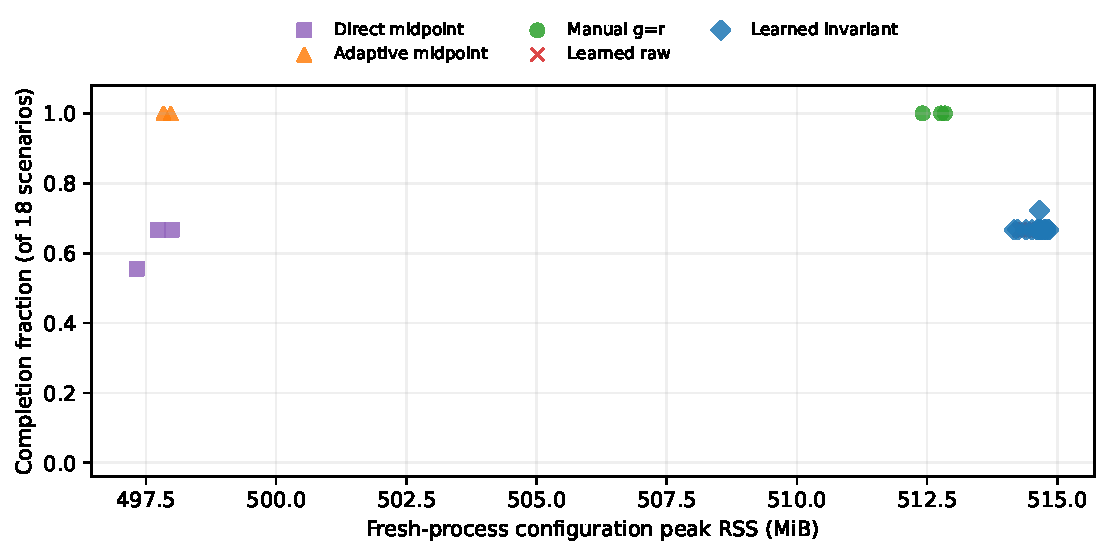
\includegraphics[width=0.95\textwidth]{fig_configuration_memory.pdf}
\caption{Completion versus historical fresh-process configuration peak
RSS. All 38 configurations are shown; the completion denominator is
18 for each. Peak RSS includes the process baseline and all trials,
including failures. It is distinct from the completed-run error
summaries used in the main accuracy--work figure and does not establish
a model-memory or deployment-efficiency advantage.}
\label{fig:configuration-memory}
\end{figure}

\section{Corrected historical checks and excluded screens}
\label{sec:historical-checks}

The historical physical-time midpoint implementation had an incorrect
Kepler-force sign, and the transformed exact-H control had detached the
Hamiltonian differentiation graph. Those outputs do not supply valid
physical evidence. Corrected implementations are retained and checked
separately. In the one-period direct-midpoint check, state errors are
0.113677, 0.0268003 and 0.00660781 at steps 0.01, 0.005 and 0.0025;
the observed orders are 2.0846 and 2.0200. These are refinement checks,
not evidence for exact energy conservation or a necessary neural
regularisation mechanism.

\begin{table}[ht]
\centering\small
\caption{All eight corrected historical Kepler configurations over
100 periods, generated from saved raw records. The frozen historical
learned monitor is a single checkpoint, distinct from the independent
deployment arms. Wall times belong to the original recorded CPU host;
field calls do not equate analytic and automatic-differentiation costs.}
\label{tab:historical-cost}
\begin{tabular}{lrrrr}
\toprule
Method & Max. energy error & Final state error & Field calls & Wall (s) \\
\midrule
Direct, $\Delta t=0.005$ & 0.0309 & 2.47 & 7.07e+05 & 5.13 \\
Direct, $\Delta t=0.0025$ & 0.00759 & 0.658 & 1.33e+06 & 10.7 \\
Adaptive, rtol=1e-06 & 0.00246 & 1.07 & 9.83e+05 & 7.5 \\
Adaptive, rtol=1e-08 & 3.29e-05 & 0.00771 & 3.33e+06 & 27.2 \\
Manual, $h=0.04$ & 0.019 & 0.0363 & 1.32e+05 & 10.9 \\
Manual, $h=0.02$ & 0.00474 & 0.00955 & 2.21e+05 & 17.9 \\
Learned, $h=0.04$ & 0.00544 & 0.366 & 3.34e+05 & 43.8 \\
Learned, $h=0.02$ & 0.00135 & 0.092 & 5.67e+05 & 75.4 \\
\bottomrule
\end{tabular}

\end{table}

At $h=0.02$, that learned monitor has lower maximum energy error than
manual $g=r$ but larger final-state error, more field calls and longer
recorded wall time. The adaptive tolerance $10^{-8}$ has the smallest
energy and final-state errors in this finite grid. The comparison
supports reporting state accuracy with energy variation, not a general
learned-monitor efficiency advantage. All eight raw records, including
angular-momentum errors, are in
\code{results/expAC2/corrected_100period.json}.

Earlier orbit-transfer work freezes one historical checkpoint. Its
primary grid contains 40 learned and 40 manual runs: the learned monitor
completes 25/40, while manual $g=r$ completes 40/40. A declared post-hoc
refinement adds 60 runs on the 15 failed scenarios, using two smaller
steps and both monitors. The later returned-residual replay of these
140 evaluations completes 106; it changes one refinement failure to
completion. The original smaller-step counts and their corrected
successors remain distinct in the stored records. Across the entire
historical returned-residual replay, 1748 attempts yield 1217 completions
and 531 failures. None of these single-checkpoint or post-hoc outcomes
is pooled with the independent-checkpoint deployment fractions.

Historical learned-H screens used unmatched architectures, objectives
or budgets, or failed the later fidelity requirements. They are retained
as provenance in the local release, not as admissible evidence for a
learned-H deployment interaction. The current gate's five rejected
candidates and absence of downstream runs remain the relevant reported
learned-H outcome. No directional-barrier theory or results enter this
manuscript.

\section{Reproducibility and release checklist}

The release package should contain the source file
\code{paper_g2_jcp_new.tex}, this supplement, the generated figure source,
the local evidence maps and machine-readable claim files. Before
submission, the authors should replace anonymous metadata, record package
versions and hardware, verify code/data URLs, rebuild all tables from the
saved raw records, and execute the complete deterministic validation suite.
The current validation executes all repository tests, the new endpoint
checks and the four result-section audits. The broader literature review
records queries, successful and failed retrievals, and reading scopes.
It supports the stated positioning without proving absence of all prior
work. The package still requires final author metadata and archival URLs.

\end{document}
